\section{Příklad 4}
% Jako parametr zadejte skupinu (A-H)
\ctvrtyZadani{H}

\vspace{1cm}
\large{\textbf{Rešení (Metoda smyčkových uzlů):}}
\vspace{0.5cm}

%%% Krok 1
\begin{center}
\textbf{Krok 1} - Vypočítáme uhlovou rychlost a impedance na cívkách a kondezátorech. \\
\end{center}
\vspace{-0.5cm}

\begin{gather*}
\omega = 2 \times \pi \times f = 2 \times \pi \times 95 = 596,9026\ rad*s^-1 \\\\
\newline
\newline
Z_{L_1} = -j \times \omega \times L_1 = j \times 596,9026 \times 0,16 = j95,5044 \Omega \\\\
\newline
\newline
Z_{L_2} = -j \times \omega \times L_2 = j \times 596,9026 \times 0,075 = j44,7677 \Omega \\\\
\newline
\newline
Z_{C_1} = -j \times \frac{1}{\omega \times C_1}  = -j \times \frac{1}{596,9026 \times 0,000155} = -j10,8085 \Omega \\\\
\newline
\newline
Z_{C_2} = -j \times \frac{1}{\omega \times C_2}  = -j \times \frac{1}{596,9026 \times 0,00007} = -j23,9331 \Omega \\\\
\end{gather*}

\newpage

%%% Krok 2
\begin{center}
\textbf{Krok 2} - Sestavíme si rovnice pro smyčkové proudy $I_A$, $I_B$, $I_C$. \\
\vspace{0.7cm}
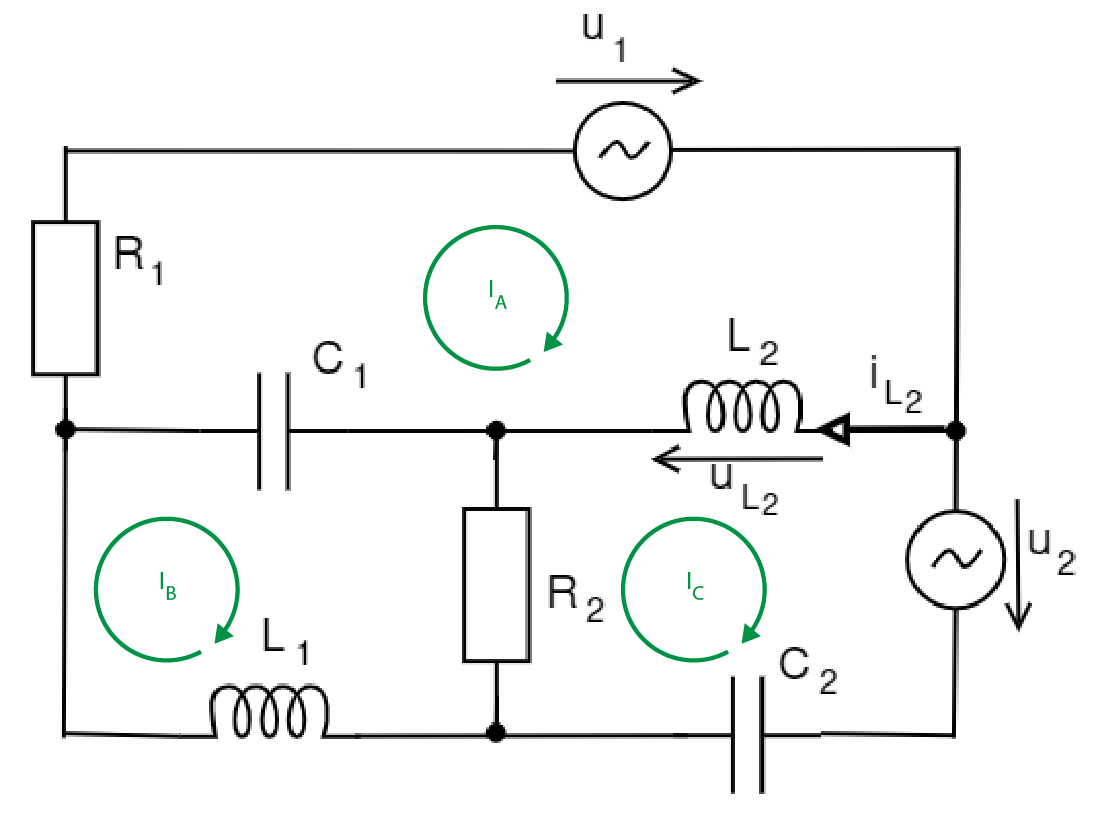
\includegraphics[scale=0.5,keepaspectratio]{fig/Pr4_steps/Pr4_step02.png}
\end{center}

\begin{gather*}
I_A: R_1 \times I_A  + U_1  + Z_{L_2} \times (I_A - I_C) +  Z_{C_1} \times (I_A - I_B) = 0 \\\\
\newline
\newline
I_B: Z_{C_1} \times (I_B - I_A) + R_2 \times (I_B - I_C) + Z_{L_1} \times I_B = 0 \\\\
\newline
\newline
I_C: Z_{L_2} \times (I_C - I_A) + U_2 + Z_{C_2} \times I_C + R_2 \times (I_C - I_B) = 0 \\\\
\end{gather*}

%%% Krok 3
\begin{center}
\textbf{Krok 3} - Vytvoříme matici ze smyčkových rovnic. \\
\end{center}

\begin{gather*}
    \begin{pmatrix}
        R_1 + Z_{L_2} + Z_{C_1} & -Z_{C_1} & -Z_{L_2} \\\\
        -Z_{C_1} & R_2 + Z_{L_1} + Z_{C_1} & -R_2 \\\\
        -Z_{L_2} & -R_2 & R_2 + Z_{L_2} + Z_{C_2} \\\\
    \end{pmatrix}
    \times
    \begin{pmatrix}
        I_A \\\\
        I_B \\\\
        I_C
    \end{pmatrix}
    =
    \begin{pmatrix}
        -U_1 \\\\
        0 \\\\
        -U_2
    \end{pmatrix}
\end{gather*}
\vspace{0.5cm}

%%% Krok 4
\begin{center}
\textbf{Krok 4} - Pomocí Cramerového a Saurussového pravidla vypočítáme $I_A$ a $I_C$. \\
\end{center}

\begin{gather*}
I_A = -0,9781 - 1,9469j A \\\\
\newline
\newline
I_C = -0,9020 - 1,7258j A \\\\
\end{gather*}

\newpage

%%% Krok 5
\begin{center}
\textbf{Krok 5} - Vypočítáme proud $I_{L_2}$. \\
\end{center}
\vspace{-0.5cm}

\begin{gather*}
\boldsymbol{I_{L_2}} = I_A - I_C = (-0,9781 - 1,9469j) - (-0,9020 - 1,7258j) = \boldsymbol{-0,0762 - 0,2211j\ A}\\\\
\end{gather*}

%%% Krok 6
\begin{center}
\textbf{Krok 6} - Vypočítáme napětí $U_{L_2}$. \\
\end{center}
\vspace{-0.5cm}

\begin{gather*}
\boldsymbol{U_{L_2}} = I_{L_2} \times Z_{L_2} = (-0,0762 - 0,2211j) \times (44,7677j) = \boldsymbol{9,8981 - 3,4113j\ V}\\\\
\end{gather*}

%%% Krok 7
\begin{center}
\textbf{Krok 7} - Vypočítáme $|U_{L_2}|$ a $\varphi_{L_2}$.. \\
\end{center}
\vspace{-0.5cm}

\begin{gather*}
\boldsymbol{|U_{L_2}|} = \sqrt{Re(U_{C_2})^2 + Im(U_{C_2})^2} = \sqrt{(9,8981)^2 + (3,4113)^2} = \boldsymbol{10,469 V} \\\\
\newline
\newline
\boldsymbol{\varphi_{L_2}} = \arctan\frac{Im(U_{C_2})}{Re(U_{C_2})} = \arctan\frac{-3,4113}{9,8981} = \boldsymbol{-0.3319
\ rad} = \boldsymbol{-19^{\circ}\ 0'\ 57.95"}
\end{gather*}

